\chapter{2D Direction finding}

\section{Introduction}
The goal of this section is to create a system that is able to determine in which direction the source of a signal is located in 2D. The equipment used is a linear microphone array, i.e. all the microphones are on the same line. There are multiple approaches to this problem, the ones discussed in this section are the fixed beamformer, MVDR and MUSIC. The implemented system should output should output a plot that shows the direction of the signal's source by the highest power value. The input should be the responses of multiple microphones.

%\subsection{Analysis}
%\paragraph{Signal model}
\section{Theory}
Every microphone records an identical but shifted audio response, and the angle that the source is located determines how much the signal is shifted between each microphone. This means that the output array of the microphones can be modeled as shifted versions of the original signal. The responses can be re-shifted back to the original position by a specific phase. If this new phase shift matches the original phase shift, the power response should be highest. This is the concept of the delay-and-form beamformer.


\begin{figure} [H]
    \centering
    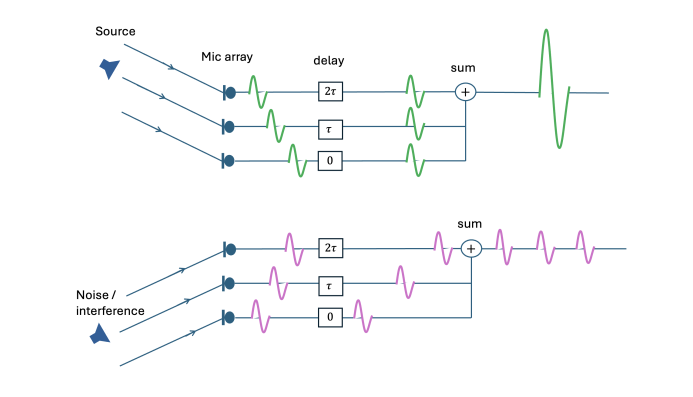
\includegraphics[width=0.9\textwidth]{docs/assignments/Midterm report/figures/module_3/Beamformer/beamformer_model.png}
    \caption{Overview of  beamformer system, as given in \cite{IP3Man}.}  
    \label{fig:beamformer_principle}
\end{figure}

The image implies that the signal can be modeled as \( \mathbf{x}(t) = \mathbf{a}(\theta)\, s(t) + \mathbf{n}(t) \). \( \mathbf{x}(t) \) is the microphone vector, \( \mathbf{s}(t) \) is the source signal, \( \mathbf{n}(t) \) is additive noise, and \( \mathbf{a}(\theta) \) is the steering vector that captures the phase shifts between microphones.

Specifically, \( \mathbf{a}(\theta) \) comprises of complex exponentials, which express the delay/phase shift of arrival of the signal at the different microphones. This phase shift/delay depends on the angle of arrival of the signal \( \mathbf(\theta) \), the spacing between the microphones, d, and the frequency of the signal f. 


Thus, as explained by \cite{IP3Man}, the steering vector \( \mathbf{a}(\theta) \) can be modeled by the following equation.
\[
 \mathbf{a}(\theta) = \begin{bmatrix}
1 \\
e^{-j(d/v)\sin(\theta)\Omega_0} \\
e^{-j2(d/v)\sin(\theta)\Omega_0} \\
\vdots \\
e^{-j(M-1)(d/v)\sin(\theta)\Omega_0}
\end{bmatrix}.
\]
\label{steering_vector_calculation}

Here, $\theta$ expresses the direction of arrival, $d$ the microphone spacing, $v$ the speed of the wave (sound in this case), and $\Omega_0$ the radial frequency.

\subsection{Beamforming principle}\label{beamf_p}
As explained earlier, the delay-and-sum beamformer aligns signals that come from a given angle $\theta$ and does not alter signals from other directions (e.g. noise in this case). Then it sums them up, so the signals from a wanted angle add up in phase (constructively), while the unwanted signals combine destructively thus becoming less important.

According to \cite{IP3Man}, for the given signal of unity power $\mathbf{x}$ and a given angle of arrival $\theta_0$, the output $y$ is
\[
y(t) = \mathbf{a}(\theta)^H \mathbf{x}(t) = \mathbf{a}(\theta)^H \mathbf{a}(\theta_0) s_0(t),
\]
and the output power is
\[
P_y(\theta) = \left| \mathbf{a}^H(\theta)\mathbf{a}(\theta_0) \right|^2 \cdot 1.
\]
In theory, by trying all the angles $\theta$, the power will be maximum when the angle tried is the same as the angle of arrival, because this is when the correct alignment happens and the signals received by the microphones are summed up in phase. However, a few assumptions are made in order to implement this approach:


\begin{itemize}
    \item It was assumed that the source is far away from the microphones. This is the far field assumption, thus the sound waves coming from the source can be taken as parallel.
    
    \item Narrow-band condition. According to \cite{IP3Man}, for the signal bandwidth B it needs to hold : \[
    B \ll \frac{v}{D}, \quad \text{where } D = (M-1)d.
    \] D here is the length of the microphone array. Because this condition does not hold for the signals of this project, a bandpass filter centered at a chosen frequency needs to be applied. This is analyzed more in the design section.
\end{itemize}

Because of the method used, there are a few factors to keep in mind that may impede the ability to obtain adequate results.

\label{beamformer_assumption_constraints}
\begin{itemize}
    \item Spatial aliasing. To avoid this, spatial sampling needs to be shorter than half the wavelength. So \[
    \Delta = \frac{d}{\lambda} < \frac{1}{2}
    \] 
    where $\Delta$ is the length measured in wavelengths, needs to be smaller than 1/2.\label{aliasing}

    \item Resolution - Aliasing tradeoff. As proven by \cite{IP3Man} and the calculations in \ref{assigment_6.2.6}, the higher the central frequency chosen, the better the resolution. This means that the lobes of the graphs are sharper. On the other hand, if the central frequency is increased too much, then the wavelength $\lambda$ becomes smaller and thus the $\Delta$ bigger which leads to aliasing. So at low frequencies, 2 lobes might be merged with each other and be indistinguishable, but in high frequencies they might be disrupted by destructive aliasing.   

\end{itemize}

\section{Design}
\subsection{Beamformer}

As proven by \cite{IP3Man}, the power of a signal \textbf{x} after beamforming is: \[
P_y(\theta) = \mathbf{a}^H(\theta) \mathbf{R}_x \mathbf{a}(\theta)
.\]
Here $\mathbf{a}$ is the steering vector and $\mathbf{R_x}$ is the auto covariance of the signal.
Thus the $\theta$ where the power is maximized is our direction of arrival.


An example of the outputs of the functions can be seen in \ref{Assignment_6.4.1}. The plots confirm the wider lobes the matched beamformer creates and as a result 2 sources are overlapping in the power spectrum.

The pipeline for applying beamforming can be seen in Fig. \ref{fig:beamformer_pipeline}. It is thus apparent that the central frequency selection and the computation of the STFT (Short Time Fourier Transform) are crucial steps. Both of these are explained in \cite{IP3Man}. The core idea is that the STFT transforms the signal into the frequency domain. It essentially decomposes the signal into separate frequency bins, where each bin represents a narrow band version of the original signal evolving over time. 

\subsubsection{Bandwidth selection}
As explained in \ref{beamf_p}, the bandwidth (B) needs to be smaller than $\frac{v}{d*(M - 1)}$. For this project, $d = 0.1 m$, $M = 6$ and $v = 343 m/s$. Thus the bandwidth (B) needs to be smaller than 686 \text{Hz}.
The formula given from \cite{IP3Man} for the effective bandwidth of each bin is : \begin{equation}
    B = \frac{f_s}{\texttt{samples per bin}}
\end{equation}
\todo{Do not use samples, but talk based on time and frequency}
More samples per bin mean lower bandwidth (B), safer narrow band assumption but lower resolution while less samples per bin mean higher bandwidth (B), worse narrow bandwidth assumption but increases resolution.
By setting the samples per bin to 256 and the sampling frequency ($f_s$) to 48 kHz, the bandwidth (B) results in 187.5 Hz, which is way smaller than 686 Hz.

\label{central_frequency_selection}
\subsubsection{Central frequency selection}
As also explained in Fig. \ref{beamf_p}, there is a tradeoff between spatial aliasing and resolution. Thus the best possible solution is to sample as close to the limit, thus close to half wavelength. This results in a central frequency close to 1715 Hz as seen in [\ref{module_3_calculation_central_frequency}]. Given the calculated B  (187.5 Hz), the best possible feasible bin frequency is 1687.5 Hz.

\subsection{MVDR}

The objective of implementing an MVDR beamformer is to choose a direction from where the source is coming and to minimize the gain of the rest of the
angles. Thus it works like a filter (the vector $\textbf{w}$ below), that lets only the signal from the wanted direction pass and attenuates the signals from other directions. This translates to two requirements that must be implemented:

\begin{equation}
\textbf{w}^\textbf{H}\textbf{a}(\theta_0)=1
\end{equation}

\noindent This constraint has a specified $\theta_0$ and the gain of the signal that comes from this angle should not be reduced, whereas the gain from all other angles should be reduced as much as possible. This results in the second constraint:

\begin{equation}
\textbf{w}_{opt}=arg\: min\:\textbf{w}^\textit{H}\textbf{R}_x\textbf{w}
\end{equation}


\noindent The solution of these two constrains results in the following:

\begin{equation}
\textbf{w}_{opt}=\frac{\textbf{R}_x^{-1}\textbf{a}(\theta)}{\textbf{a}^\textit{H}(\theta)\textbf{R}_x\textbf{a}(\theta)}
\end{equation}
\label{MVDR_beamformer}

\noindent The power response of the system will be the output:

\begin{equation}
    P_y(\theta)=\textbf{w}^\textit{H}\textbf{R}_x\textbf{w}=\frac{1}{\textbf{a}^\textit{H}(\theta)\textbf{R}_x^{-1}\textbf{a}(\theta)}
\end{equation}

\subsection{MUSIC}
As explained by \cite{IP3Man}, when there are many sources, the signal \textbf{X} can be modeled as:
\begin{equation}
\mathbf{X} = \mathbf{A}\mathbf{S} : M \times N, \quad
\mathbf{A} = [\mathbf{a}_0 \ \mathbf{a}_1 \ \cdots \ \mathbf{a}_Q] : M \times Q, \quad
\mathbf{S} = \begin{bmatrix} 
\mathbf{s}_0 \\ 
\mathbf{s}_1 \\ 
\vdots \\ 
\mathbf{s}_Q 
\end{bmatrix} : Q \times N \\
\end{equation}

Here $M$ is the number of microphones, $Q$ is the number of sources and $N$ is the number of samples.




Because the columns of \textbf{X} are linear combinations of the vectors inside \textbf{A}, the rank of \textbf{X} will be the number of sources Q. This can be verified by an example (\ref{fig:assignment_7.1.4_plot}).

As shown in \cite{IP3Man} and in Fig. \ref{fig:SVD_interpretation}, the dominant singular vectors of the matrix \textbf{U} span the same subspace as the matrix \textbf{A}, but orthogonally. Additionally, the singular vectors that are really small (zero) span the subspace of the noise \textbf{$U_n$}.
$$
\mathbf{X} = \mathbf{A}\mathbf{S}, \qquad \mathbf{X} = \mathbf{U}\Sigma\mathbf{V}^H.
$$

The matrix \textbf{U} comprises of the matrix \textbf{$U_s$} which contains the dominant singular vectors that span the signal and are equal to the number of sources Q, and the matrix \textbf{$U_n$} whose vectors span the noise subspace.

As a result, because \textbf{A} and \textbf{$U_s$} are the same and \textbf{$U_n$} is orthogonal to \textbf{$U_s$}, if a steering vector $\mathbf{a}(\theta)$ points to an angle where there is a source (so this steering vector belongs to \textbf{A}), \textbf{$U_n$} will be orthogonal to it.


The formulae below express these properties to help in finding the direction of arrival.
$$
P_{\text{music}}(\theta) = \frac{1}{\mathbf{a}^H(\theta)\mathbf{U}_n\mathbf{U}_n^H\mathbf{a}(\theta)}, \qquad \theta \in [-\pi/2, \pi/2].
$$

$$
\mathbf{a}(\theta_0) \perp \mathbf{U}_n \quad \Rightarrow \quad \mathbf{U}_n^H\mathbf{a}(\theta_0) = \mathbf{0} \quad \Rightarrow \quad \mathbf{a}^H(\theta_0)\mathbf{U}_n\mathbf{U}_n^H\mathbf{a}(\theta_0) = 0.
$$
So there will be peaks in the spectrum when the angle is one of the source angles.

Thus the only thing to find from \textbf{X} is the noise subspace \textbf{$U_n$}. This can be found either from the SVD or from the eigen decomposition of the auto covariance $R_x$. As proven in \cite{IP3Man}, the eigenvectors of $R_x$ are the same as the left singular vectors of \textbf{X}.

\section{Test results}
\subsection{Beamformer}
\label{beamformer_testing}
Four configurations were used to acquire measurements to test all the algorithms. The configurations all included an array of six microphones and one or two speakers.  The first three configurations included a single speaker that was placed at three different angles, one was placed 7.4 meters in front of the microphones (at an angle of zero degrees). In the second configuration the speaker was placed at an angle of 30 degrees and in the third configuration it was placed at an angle of 60 degrees. The fourth configuration contained two sources placed at +7$^\circ$ and -7$^\circ$. During the tests, the speakers were playing white noise, this was done to be able to select frequency slices while processing the data of the measurement to compare the results at different frequencies.


\subsubsection{One source} For one source at $0^\circ$, the beamformer performs satisfactory. There is an absolute error of $0.45^\circ$.

\begin{figure} [H]
    \centering
    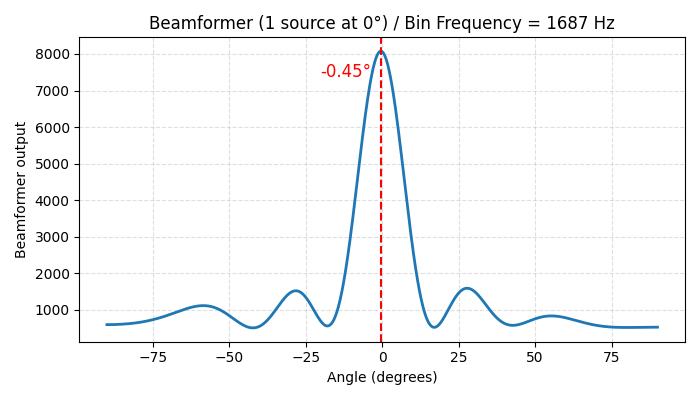
\includegraphics[width=0.8\textwidth]{docs/assignments/Midterm report/figures/module_3/Beamformer/Beamformer 1 source/Beamformer_0.png}
    \caption{Beamformer at 0$^\circ$.}  
    \label{fig:beamformer_0_degrees}
\end{figure}

The $30^\circ$ plot shown in Fig. \ref{fig:beamformer_30_degrees} shows that the accuracy is as desired.
The $60^\circ$ plot as shown in Fig. \ref{fig:beamformer_60_degrees} shows there is an offset of around $2^\circ$. This might be because the speaker was not placed at exactly $60^\circ$. Moreover, the angle to the speaker in the setup is measured from the middle of the array, while in \ref{fig:beamformer_principle}, the angle is taken from the first microphone of the array.


\subsubsection{Two sources}

\label{beamformer_resolution_2_sources_problem}
As explained in \ref{beamformer_assumption_constraints}, there is a tradeoff between spatial aliasing and resolution. If there are 2 sources in a signal, the final power spectrum plotted for the beamformer is practically the sum of the power spectrum for each source as if they were received as different signals. If the central frequency is lower, each of the lobes is thicker/more spread out. Thus the peak of their sum is somewhere in between, and the 2 sources are indistinguishable. This can be seen in the Fig. \ref{fig:beamformer_2_source_1687Hz}.

\begin{figure} [H]
    \centering
    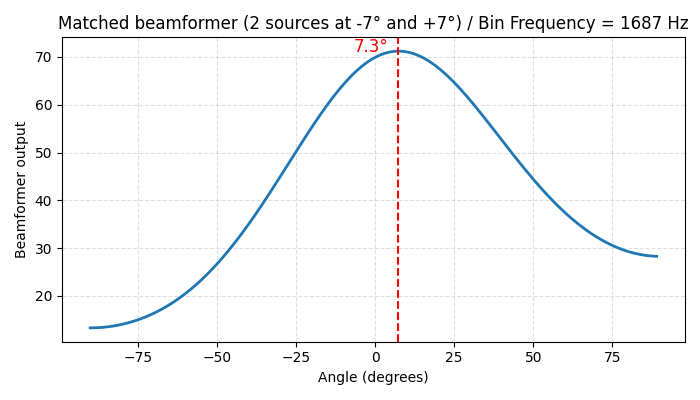
\includegraphics[width=0.8\textwidth]{docs/assignments/Midterm report/figures/module_3/Beamformer/Beamformer 2 source/Beamformer_1687Hz.png}
    \caption{Beamformer at +7$^\circ$, -7$^\circ$, low resolution.}  
    \label{fig:beamformer_2_source_1687Hz}
\end{figure}

If the central frequency is higher, the lobes created by the 2 sources are sharper and are not merged in one thick lobe. Thus there are 2 peaks but also spatial aliasing.In this case it is known that the 2 peaks seen are not result of aliasing. In lower frequencies as in \ref{fig:beamformer_2_source_1687Hz}, the peak of the power is around the center of the graph. Thus most of the signal lies there. As a result, it it known that the peaks caused by the 2 sources will occur in that region. The plot was expected, as 2 peaks are visible but they are still merged, justifying the operation of the beamformer. This is also justified in \ref{Assignment_6.4.1}, where there are 2 sources at  $0^\circ$ and $15^\circ$ by using a simulated signal.  

\begin{figure} [H]
    \centering
    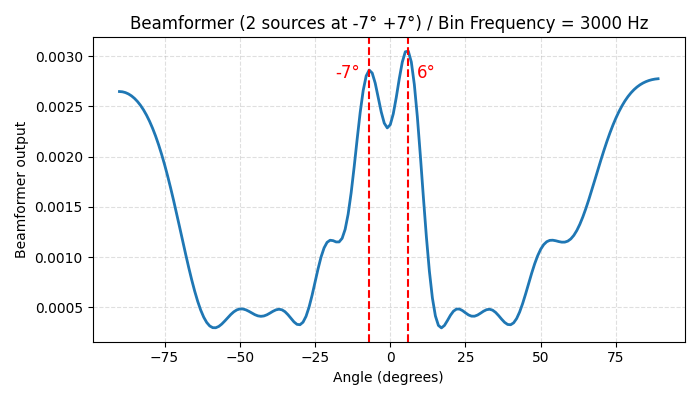
\includegraphics[width=0.8\textwidth]{docs/assignments/Midterm report/figures/module_3/Beamformer/Beamformer 2 source/Beamformer_3000Hz.png}
    \caption{Beamformer at +7$^\circ$, -7$^\circ$, higher resolution.}  
    \label{fig:beamformer_2_source_3000Hz}
\end{figure}


\subsection{MVDR}
The configuration for testing is the same for all algorithms, which is explained in \ref{beamformer_testing}.

\subsubsection{One source} 
The graph obtained from the measurements of the setup where the speaker was placed at $0^\circ$ can be seen below. The peak seen in the plot shows that the angle of the signal's source was placed at an angle of $-1^\circ$. This is a sufficiently accurate result as the speaker was probably not \textit{exactly} placed at an angle of $0^\circ$ for the measurement. It is reasonable to assume that most of the measurements have an offset like this that is due to the imperfect placing of the speakers and the microphones. Another factor that can contribute to an unideal response is the reflection of sound from other objects in the room or the walls.

\begin{figure} [H]
    \centering                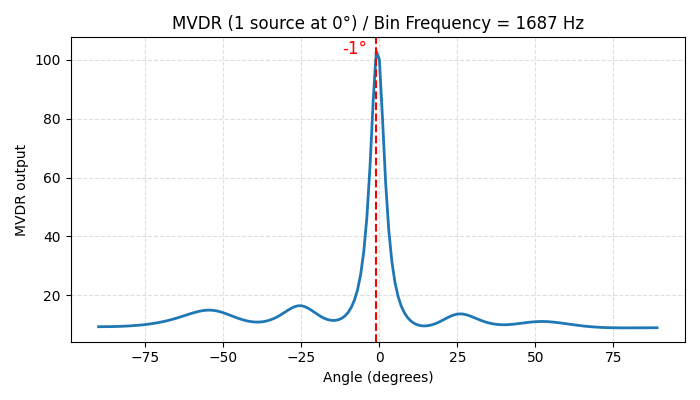
\includegraphics[width=0.8\textwidth]{docs/assignments/Midterm report/figures/module_3/MVDR/MVDR 1 source/MVDR_0.png}
         \caption{single source at 0 degrees}
         \label{fig:MVDR_0_degrees}
     \end{figure}


The plot obtained after changing the angle of the source to $30^\circ$, shown in Fig. \ref{fig:MVDR_30_degrees}, peaks at $\theta=30^\circ$. This is also a good accuracy.

The graph acquired after measuring the response of the microphones with the source placed at $\theta=60^\circ$, shown in Fig. \ref{fig:MVDR_60_degrees}, shows the peak at about $60^\circ$. 



\subsubsection{Two sources} 
The fourth measurement configuration included two speakers placed in front of the microphone array. One of them was placed at an angle of $7^\circ$, the other one was placed at $-7^\circ$. As explained earlier in this chapter (\ref{aliasing}), when $\Delta$ surpasses $\frac{1}{2}$, spacial aliasing occurs. Because the frequency selected for this measurement was 3000 Hz instead of the previously used 1687 Hz, $\Delta$ surpassed $\frac{1}{2}$ (as $\Delta=\frac{d}{\lambda}$ and $\lambda=\frac{v}{f}$). The aliasing is visible on the ends of the graph obtained during this measurement (see Fig. \ref{fig:MVDR_2_sources}).

\begin{figure} [H]
    \centering
    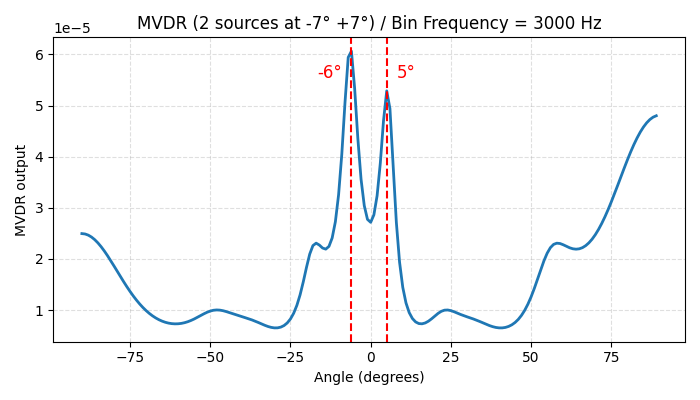
\includegraphics[width=0.7\textwidth]{docs/assignments/Midterm report/figures/module_3/MVDR/MVDR 2 source/MVDR_7_-7.png}
    \caption{MVDR at $60^\circ$.}  
    \label{fig:MVDR_2_sources}
\end{figure}


These responses show that when comparing the response of an MVDR beamformer with a fixed beamformer response, the heights of the sidelobes compared with the main lobe appear significantly lower. These graphs also show that the main lobe of an MVDR is much narrower when compared to the main lobe in the response of a fixed beamformer, making it much easier to determine the angle of the source. In short, these MVDR responses tell us that it is more accurate than the matched beamformer in finding the angle of the source location. 

\subsection{MUSIC}

\subsubsection{One source}
For one source the results of the MUSIC were satisfactory.

\begin{figure} [H]
    \centering
    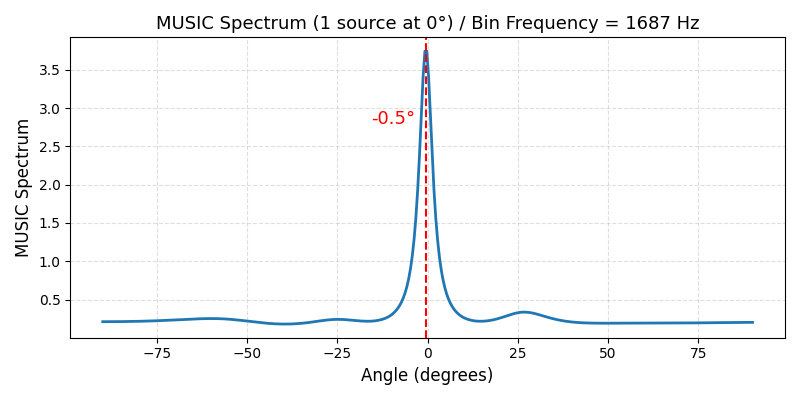
\includegraphics[width=0.8\textwidth]{docs/assignments/Midterm report/figures/module_4/MUSIC/MUSIC Single Source/Music_0_degrees.png}
    \caption{MUSIC at 0$^\circ$, higher resolution.}  
    \label{fig:music_1_source_0_degrees}
\end{figure}



It is apparent that the lobe is really sharp, exactly because of the way the MUSIC works. There is a small offset of 0.5$^\circ$, but this can be due to setup errors. 

The plot for $30^\circ$ can be seen in Fig. \ref{fig:music_1_source_30_degrees}. There is also a really small offset of $0.3^\circ$, but given its magnitude it is not that significant.

The plot for $60^\circ$ can be seen in Fig. \ref{fig:music_1_source_60_degrees}. A larger offset of $4.82^\circ$ is visible. This is due to having a finite amount of samples, because, as explained in \cite{IP3Man}, MUSIC's resolution depends on the number of samples N. Also aliasing has started to appear. Aliasing is logical because with the chosen central frequency, we are on the verge of aliasing as explained in Fig. \ref{central_frequency_selection}. Also, it is clear that aliasing does not have a significant influence, because it happens only on the sides of the graph.



\subsubsection{Two Sources}
For 2 sources the situation for MUSIC is similar to the results for MVDR (\ref{beamformer_resolution_2_sources_problem}) and can be seen in \ref{fig:music_2_source_1687}. So there needs to be a higher central frequency for the peaks to separate.



This is seen with 3185.5 Hz. 
\begin{figure} [H]
    \centering
    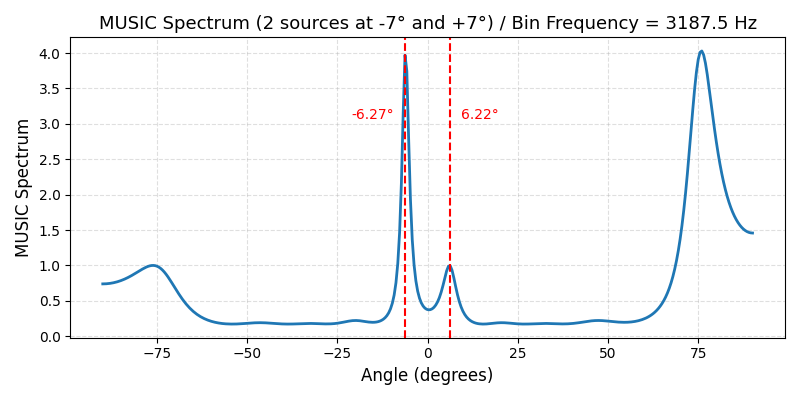
\includegraphics[width=0.8\textwidth]{docs/assignments/Midterm report/figures/module_4/MUSIC/MUSIC 2 sources/Bin freq = 3185.5.png}
    \caption{Beamformer at +7$^\circ$, -7$^\circ$, higher resolution.}  
    \label{fig:music_1_source_0_degrees}
\end{figure}

The peak on the right is due to spatial aliasing and is not the actual signal. This is because, in lower frequencies [\ref{fig:music_2_source_1687}], the most "power" is concentrated in the center. Thus the area to search while increasing the frequency is the area that the big lobe takes at [\ref{fig:music_2_source_1687}].

It can be seen that with high enough frequency, MUSIC lobes are really sharp and the accuracy is impeccable with less than a degree of error per side.


When comparing the MUSIC responses to those of the MVDR, the differences are more or less identical to the differences between the MVDR and the fixed beamformer. The response of the MUSIC spectrum shows that the size of the sidelobes has dropped even further and the width of the main lobes has become even slimmer.



\section{Conclusion}

The MVDR beamformer gives a sharper and more accurate spatial response than the conventional beamformer, but its output contains more ripple. This is because MVDR suppresses signals coming from directions other than the source, which leads to narrower peaks and deeper nulls. The conventional beamformer has a smoother response and broader peaks, which makes it more suitable for single-source situations. The same behavior is observed for both the single-source and two-source measurements. Thus the MVDR is more suitable for 2 sources. 

For testing, the recordings that were made in the last year were used, as advised by the professors. However, there were similar recordings made this year, which seem to have more noise. They can be seen in Fig. \ref{module_3_recordings}. Recordings where made for one source for a variety of angles between $0^\circ$ and $60^\circ$. For 2 sources the same happened with the sources being from $+60^\circ$ and $-60^\circ$ to $+20^\circ$ and $-20^\circ$.
Both algorithms performed with an offset up to $5^\circ$ in the single source estimations, which is satisfactory taking into account the fact that there were a narrow walls which would cause signal reflections.
However in the 2 source estimates, exactly because of the signal reflections, the signals coming from the 2 sources interfere with each other as they get reflected thus causing the accuracy to drop by a lot.

Overall other factors that could have affected the results are people talking, other noise form outside and inaccurate setup of the equipment.

It is clear that MUSIC is more accurate than the other 2 algorithms previously discussed. The peaks are more sharp, thus indicating better where the signal is coming from. As in the previous modules, the recordings that were made in the last year were used, as advised by the professors. However, there were similar recordings made this year, which seem to have more noise. They can be seen in \ref{module_4_recordings}. As the 2 previous algorithms MUSIC performs better in one source estimation, and even better than MVDR and matched beamformer. However when it comes to 2 sources, the results were not satisfactory. Factors that could have affected the results are people talking, other noise form outside, inaccurate setup of the equipment and obviously and most importantly, reflections of each of the signals to the walls

\chapter{3D direction finding and integration}
\section{Introduction}
The final goal of this project is to be able to localize the valves in the heart. This must be done in 3D instead of the 2D model that was discussed in the previous chapter. This means that the existing algorithms (MVDR and MUSIC) need to be adapted to work in 3D.
To achieve this, in addition to the angle in horizontal plane, the elevation angle is also needed. Also, the far field assumption does not hold. The valves (sources) are close to the microphone array, so each microphone sees the source from a different angle.
The microphone array consists of 6 microphones placed in a 3x2 matrix, where the distance between adjacent orthogonal microphones is 5cm.

\section{Design}

% --- Paraphrased summary + equations (based on your screenshot) ---

\subsection{Near-field steering vector}
To move from a far-field model (direction vectors $a(\theta)$) to a location-based model,
we describe the source position in Cartesian coordinates:
\[
\mathbf{z} = [x,\;y,\;z]^{\mathsf T},
\]
and the $m$-th microphone position as
\[
\mathbf{z}_m = [x_m,\;y_m,\;z_m]^{\mathsf T}, \qquad m = 0,\dots,M-1.
\]
We then define a steering (direction) vector that depends on the \emph{source location}:
\begin{equation}
\mathbf{a}(\mathbf{z})
=
\begin{bmatrix}
\vdots\\[2pt]
\dfrac{1}{r_m(\mathbf{z})}\,e^{-j\omega\,\tau_m(\mathbf{z})}\\[2pt]
\vdots
\end{bmatrix},
\qquad
r_m(\mathbf{z}) = \lVert \mathbf{z}-\mathbf{z}_m\rVert,
\qquad
\tau_m(\mathbf{z}) = \dfrac{r_m(\mathbf{z})}{v}.
\label{eq:nearfield_steering}
\end{equation}

Here, $r_m(\mathbf{z})$ is the distance from the source to microphone $m$ and
$\tau_m(\mathbf{z})$ is the corresponding propagation delay (with propagation speed $v$). The factor $1/r_m(\mathbf{z})$ acts as a distance-dependent attenuator.

\subsection{Coordinate convention.}
We use the coordinate system where $x,y$ span the horizontal/vertical plane (for a standing person),
and $z$ denotes depth (into the body). The origin is chosen at the microphone array center.



For MVDR, we scan the possible \(\mathbf{z} = [x,\;y,\;z]\)
using
\begin{equation}
P_{\mathrm{mvdr}}(\mathbf{z})
= \frac{1}{\mathbf{a}^H(\mathbf{z})\, \mathbf{R}_x^{-1}\, \mathbf{a}(\mathbf{z})}.
\label{eq:Pmvdr}
\end{equation}

For MUSIC, the scan function is
\begin{equation}
P_{\mathrm{music}}(\mathbf{z})
= \frac{1}{\mathbf{a}^H(\mathbf{z})\, \mathbf{U}_n\, \mathbf{U}_n^{H}\, \mathbf{a}(\mathbf{z})}.
\label{eq:Pmusic}
\end{equation}

Summarizing, instead of scanning over possible angles, scanning is done per 3D point.
Explicitly, a range of points in the x and y direction is defined. Then the z component is varied and a plot of the power measured is made each time. The correct z component is the one that gives the maximum power out of all plots.
\label{depth_analysis}

\section{Testing}
As explained in \ref{ways_of_testing}, there are 3 possible ways to validate the design :
\begin{itemize}
    \item Simulation, where the acoustic signal received by the microphones is generated.
    \item Phantom model recordings. 
    \item Recordings of a persons heart.
\end{itemize}
Simulation and phantom model can be used with the sources playing white noise or a heartbeat. The recordings of a persons heart only include heartbeat signals.

\subsection{Frequency selection}
As explained in \ref{beamformer_assumption_constraints}, there is a theoretical upper limit on the frequency of the signal that can be selected. In addition when the signal travels through human tissue or foam instead of air, it seems to be heavily attenuated for higher frequencies as it can be seen in the amplitude-frequency plot of a heart beat signal \ref{fig:amplitude_frequency_plot}. As a result the lowest frequency possible was always chosen for the rest of the analysis.

\subsection{Simulation}
Simulation allows to verify that the localization algorithm works properly as the location of the sources can be specified when generating the audio files that simulate the heart beat. Both MVDR and MUSIC were tested. The depth of the sources was set to 0.15m.
Some representative samples are presented below, all of them exist on \ref{assignment_9.2}.
\begin{figure} [H]
    \centering
    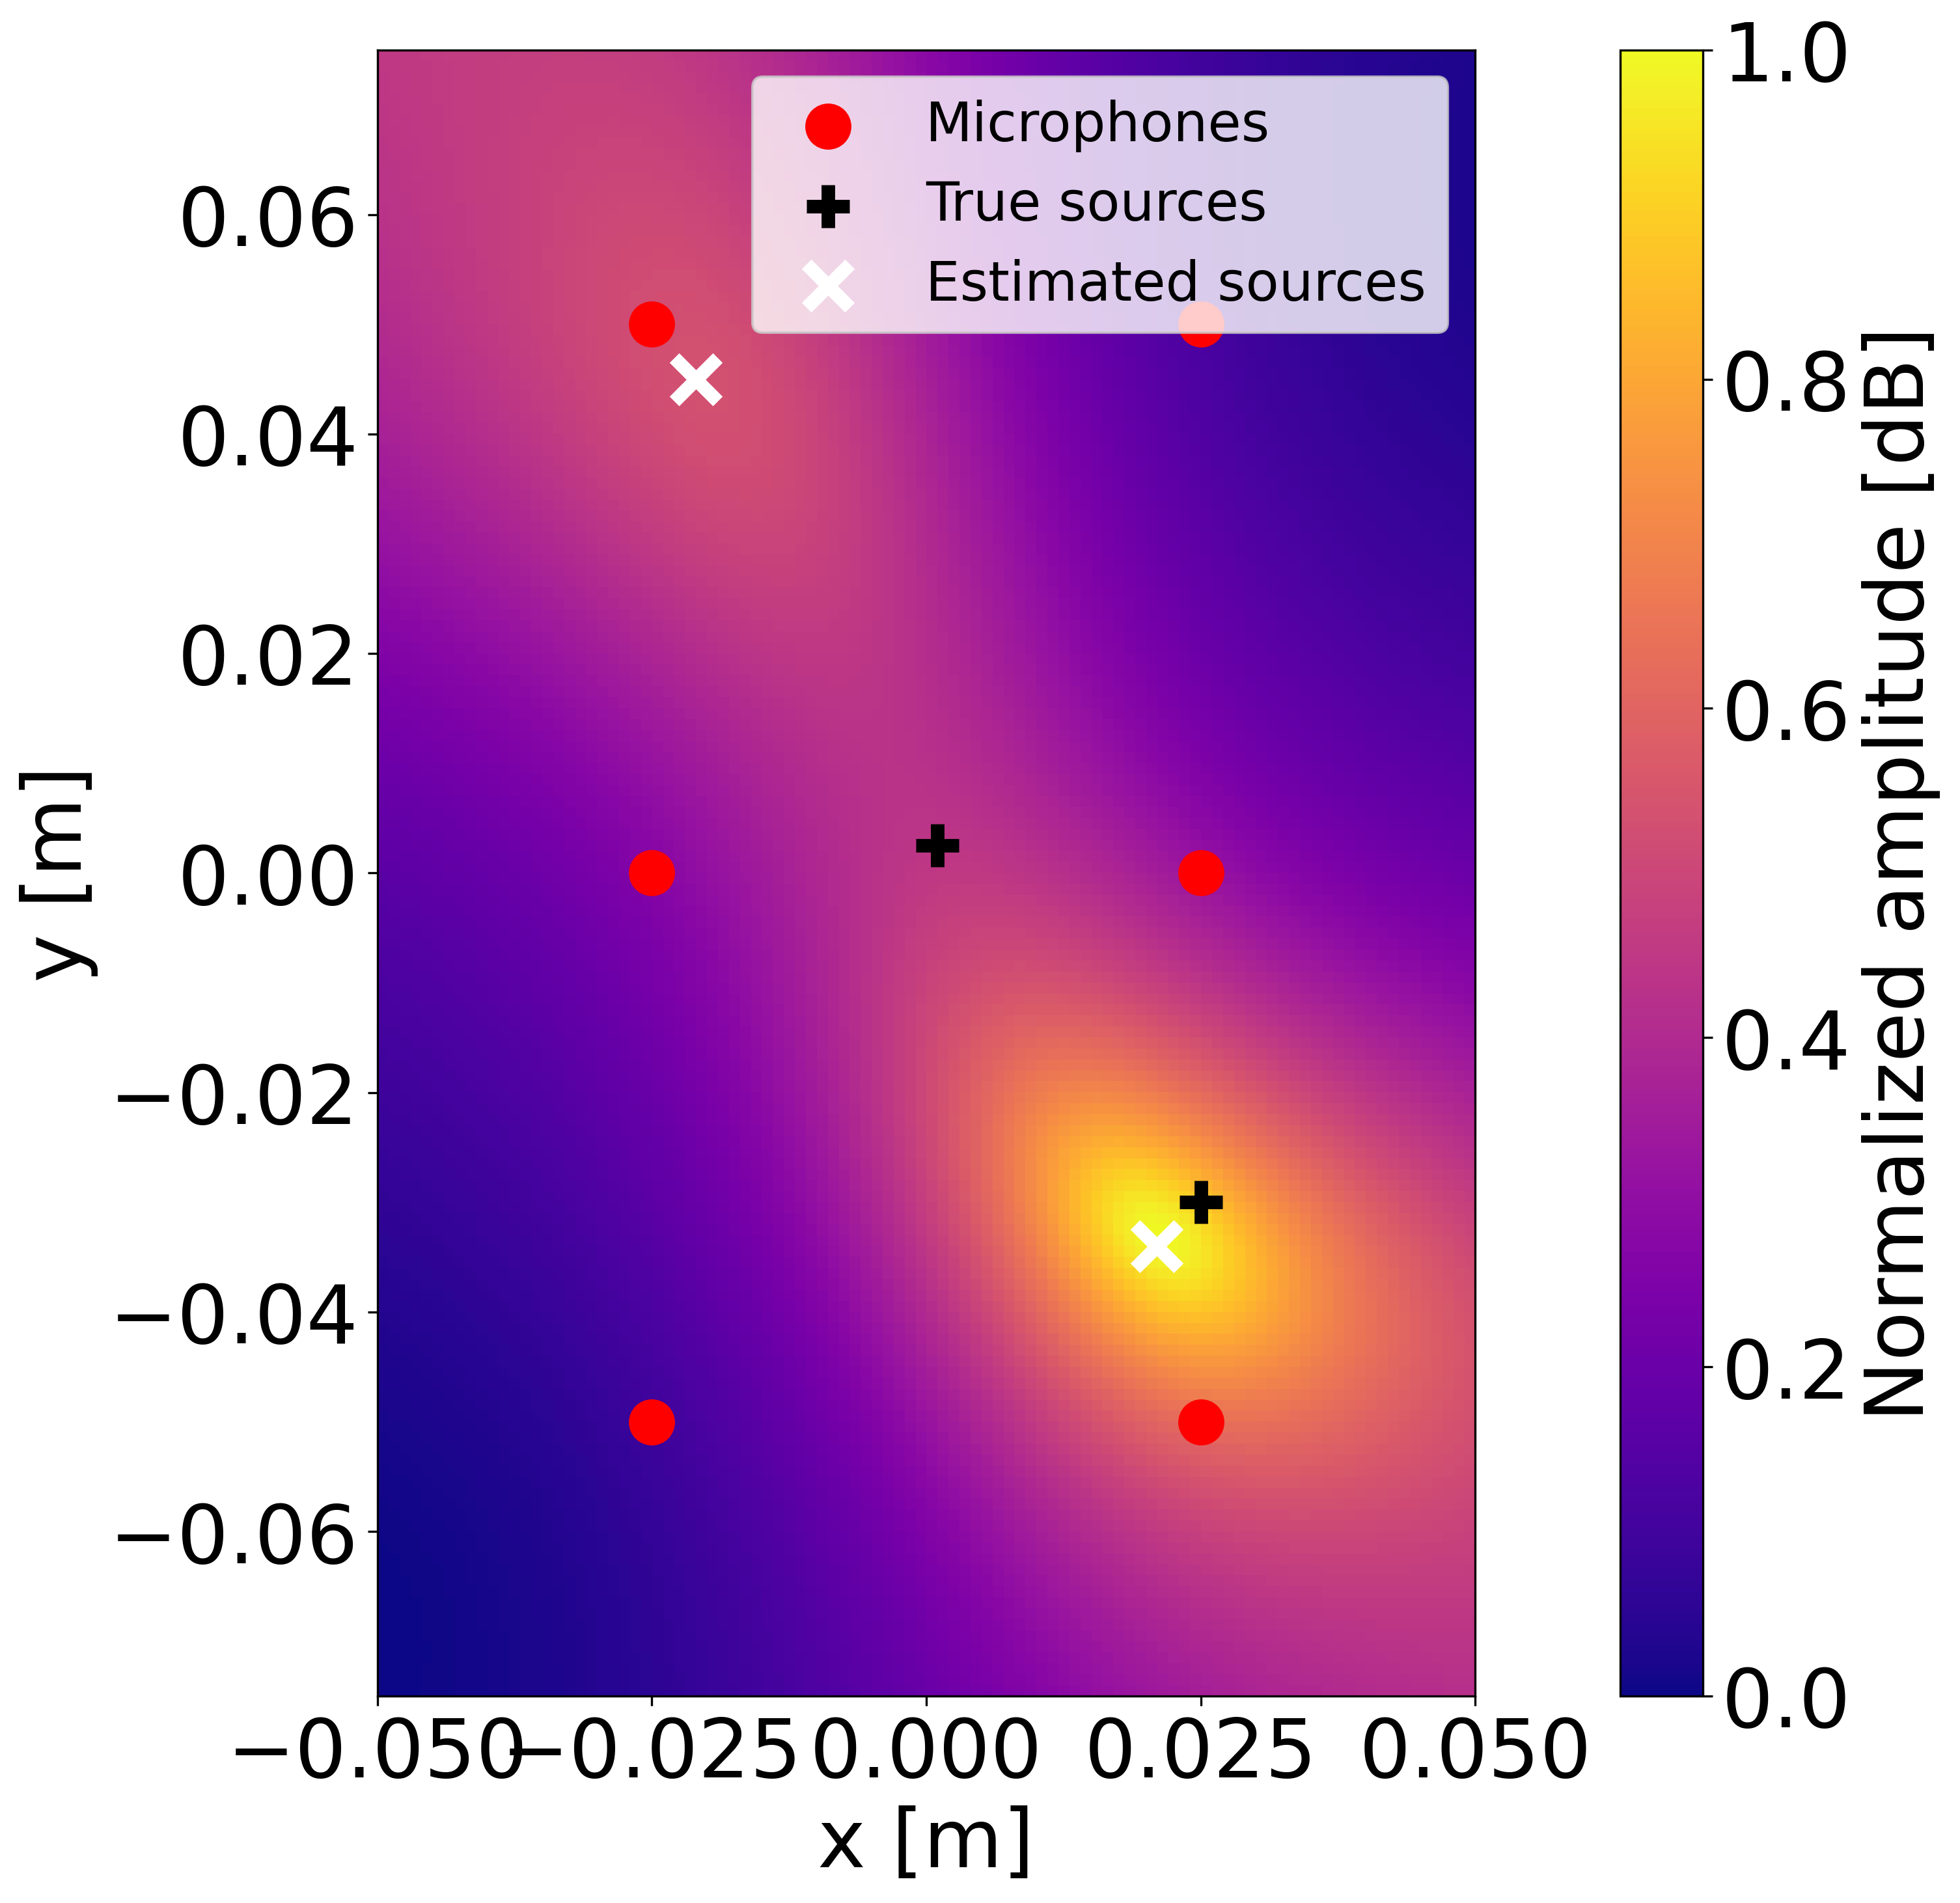
\includegraphics[width=0.6\textwidth]{docs/assignments/Final report/figures/figures/Localization/NEW/SimulationLocalizationPlots/Generated_S2_sounds---_bin0_z0.07_Fs48000_Q2_M6_v_sound340_d0.1_resolution0.001_modemusic_neighbourhood3.png}
    \caption{Power plot at a depth of 0.07m using the MUSIC algorithm with 2 simulated sources simulating the S2 peak.}  
    \label{fig:music_3D_2sources}
\end{figure}

\begin{figure} [H]
    \centering
    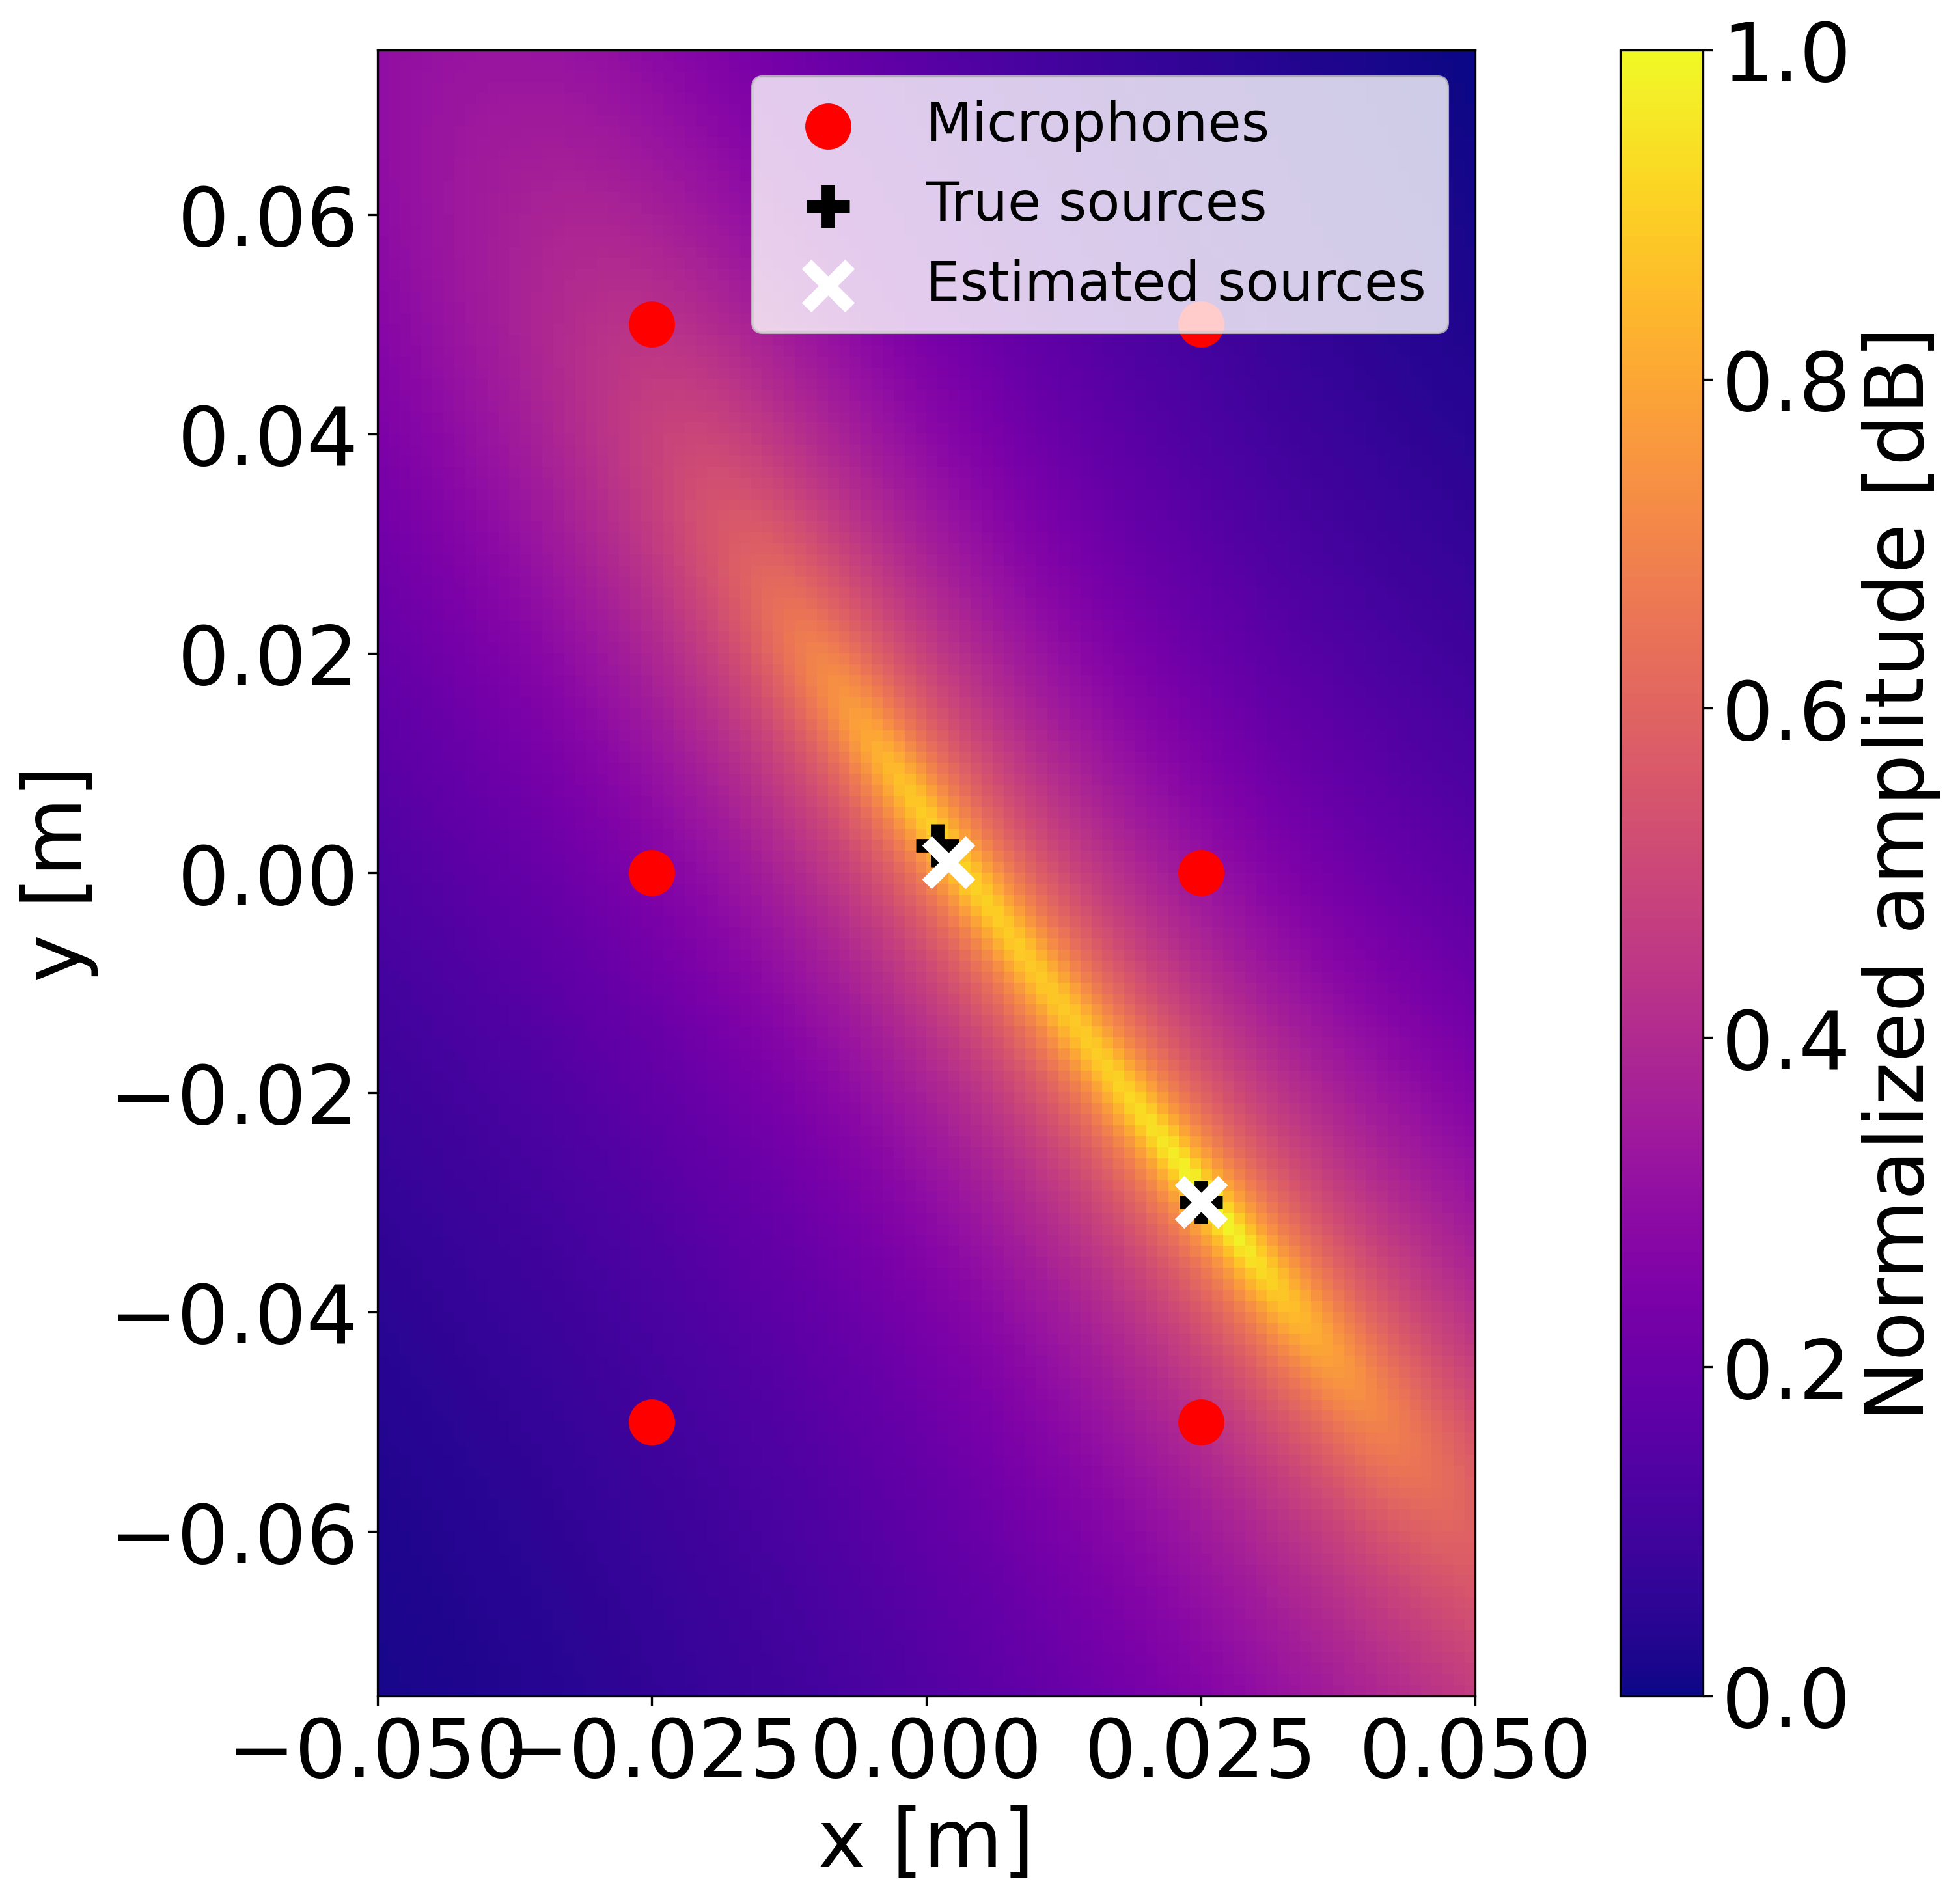
\includegraphics[width=0.6\textwidth]{docs/assignments/Final report/figures/figures/Localization/NEW/SimulationLocalizationPlots/Generated_S2_sounds---_bin0_z0.16_Fs48000_Q2_M6_v_sound340_d0.1_resolution0.001_modemvdr_neighbourhood25.png}
    \caption{Power plot at a depth of 0.16m using the MVDR algorithm with 2 simulated sources simulating the S2 peak.}  
    \label{fig:mvdr_3D_2sources}
\end{figure}

In the plots it becomes clear that the MVDR algorithm localizes the sources more accurately. The MUSIC algorithm comes to a depth of 0.07m, which is smaller than the set depth. 


\subsection{Phantom Model}
The phantom model is a step closer to reality as there is an actual recording made, in which noise is naturally added. The ability to know the exact location of the sources is maintained, as it is assumed that all the sound comes from 2 holes below the foam. The results presented here come from recordings that were made with calibration of the microphones. For the ones without calibration see \ref{phantom_rest}.

\begin{figure} [H]
    \centering
    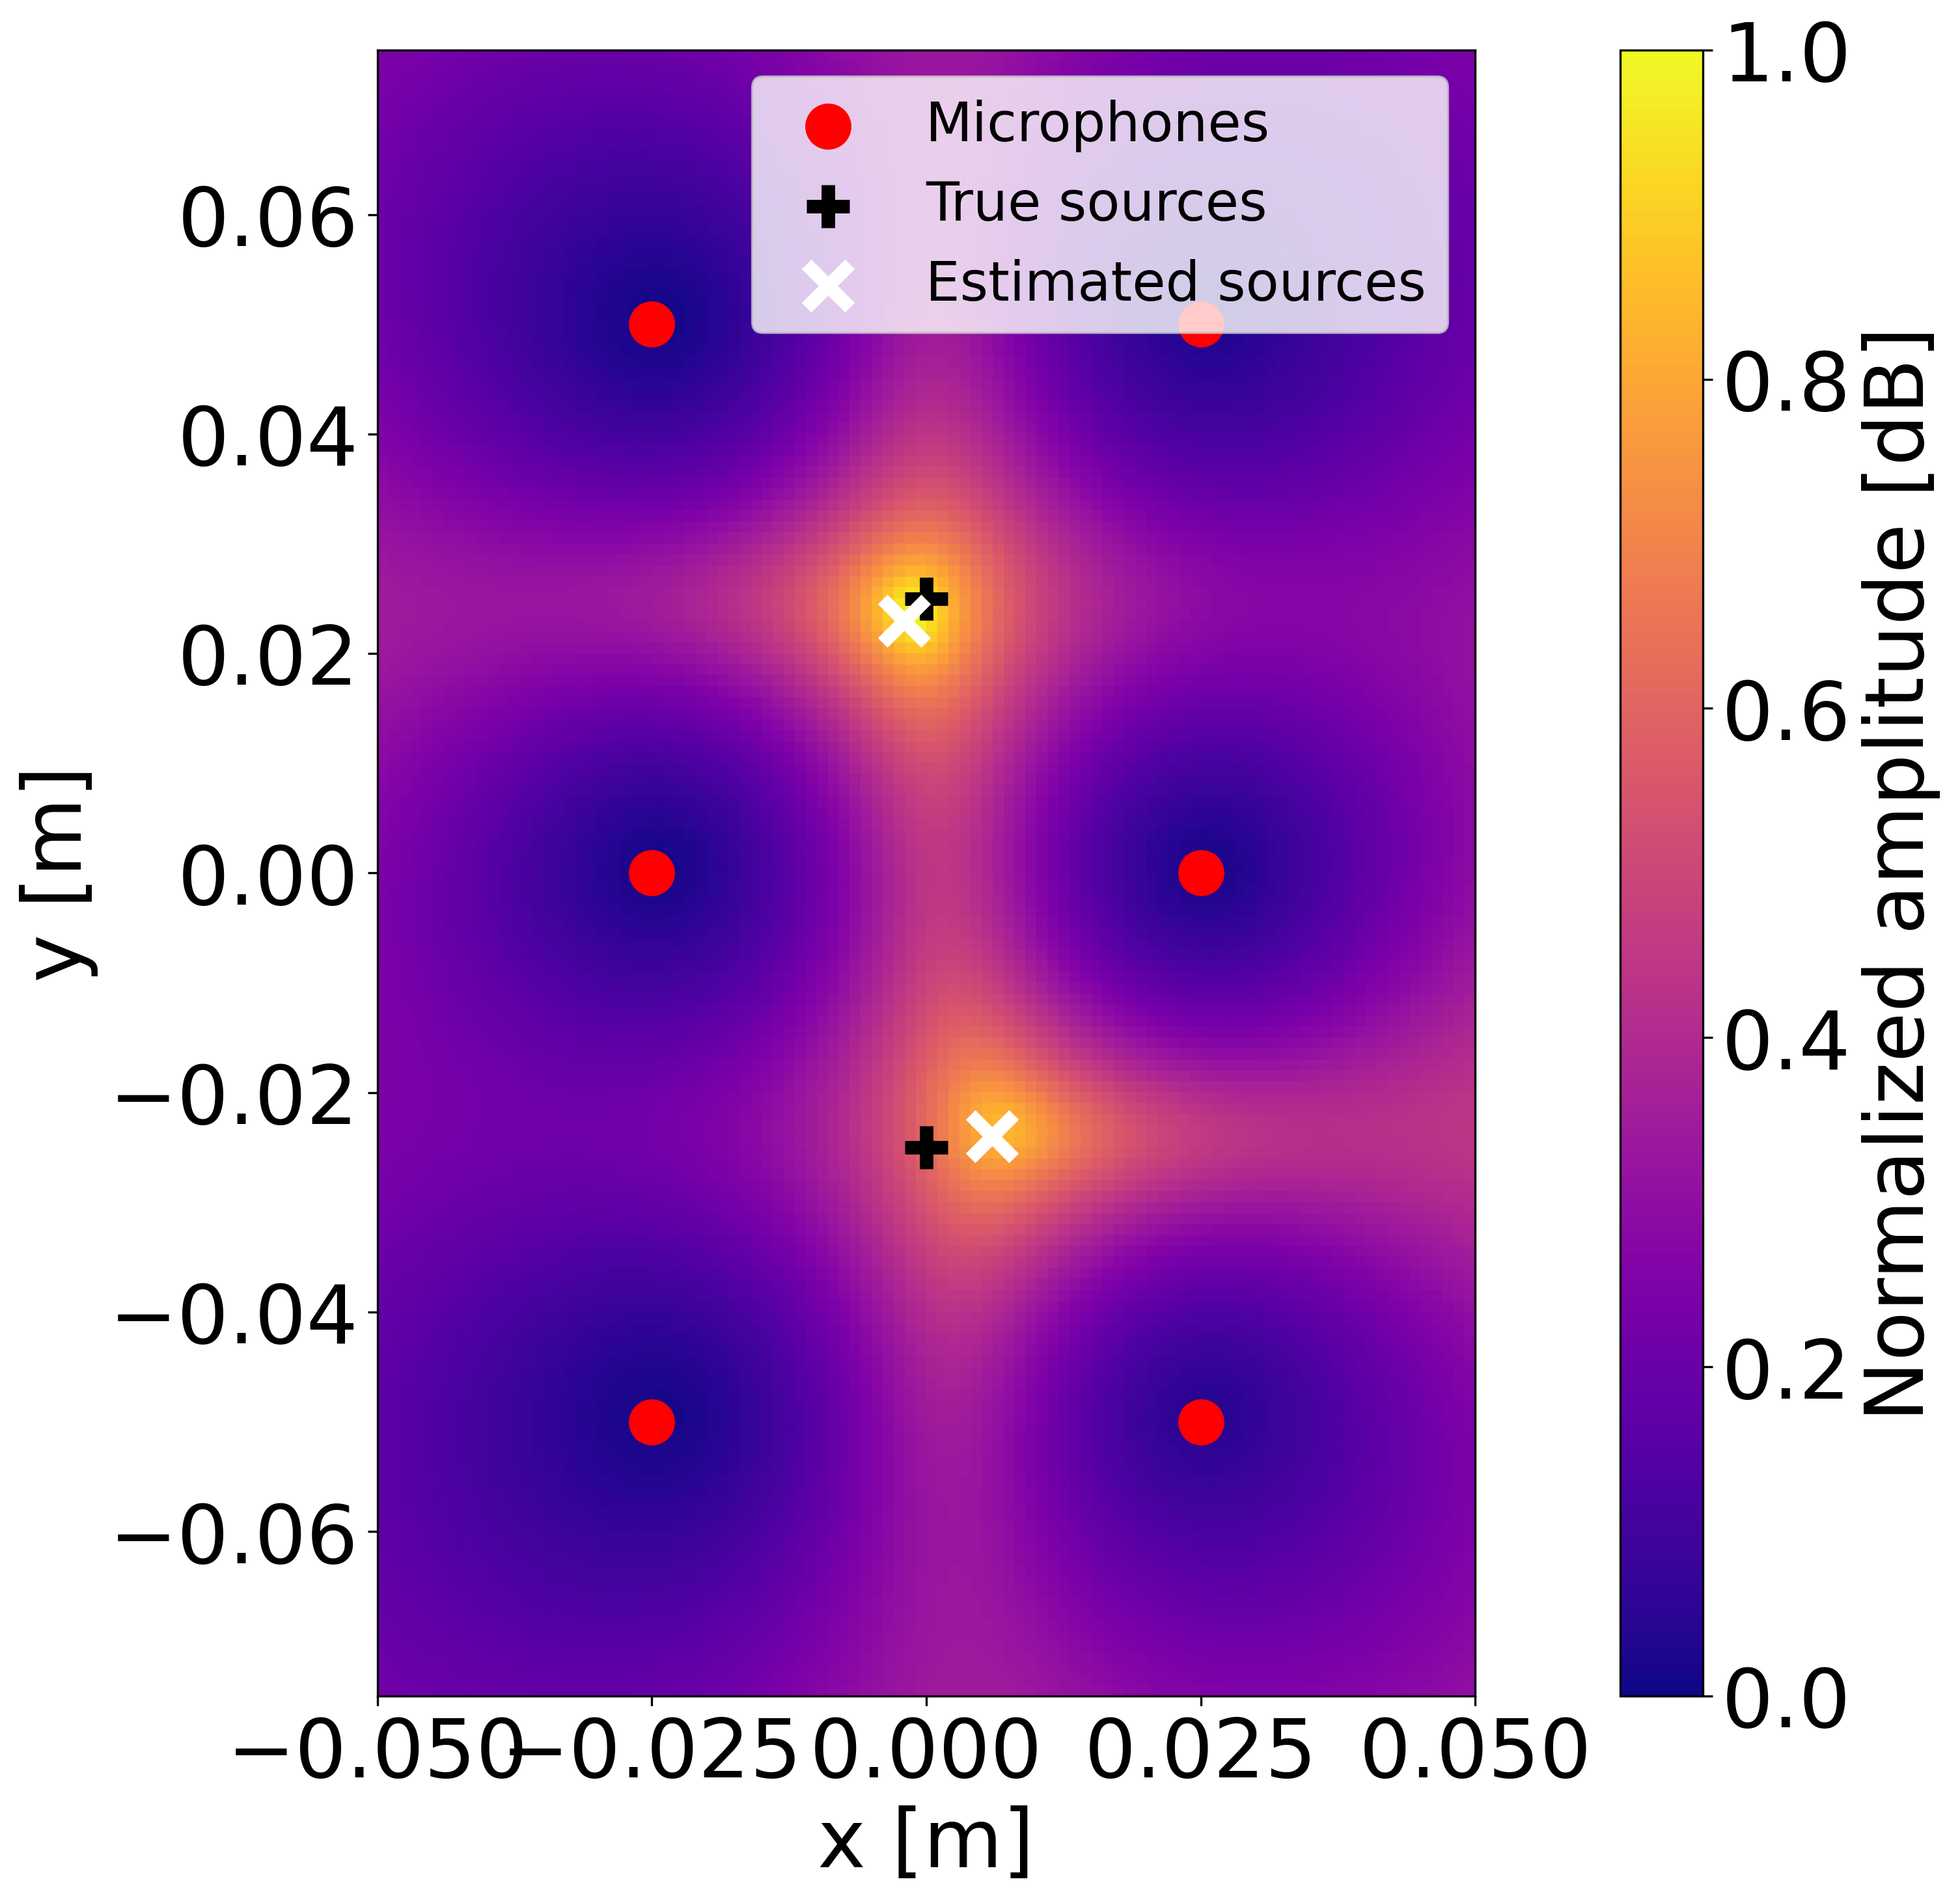
\includegraphics[width=0.6\textwidth]{docs/assignments/Final report/figures/figures/Localization/NEW/Localization_results/Calibrated_MT---_bin0_z0.0001_Fs48000_Q2_M6_v_sound340_d0.1_resolution0.001_modemusic_neighbourhood3.png}
    \caption{Power plot of the phantom model using 2 sources to simulate the S1 peak using the MUSIC algorithm at a depth of 0.0001m.}  
    \label{fig:music_3D_2sources_phantom}
\end{figure}

\begin{figure} [H]
    \centering
    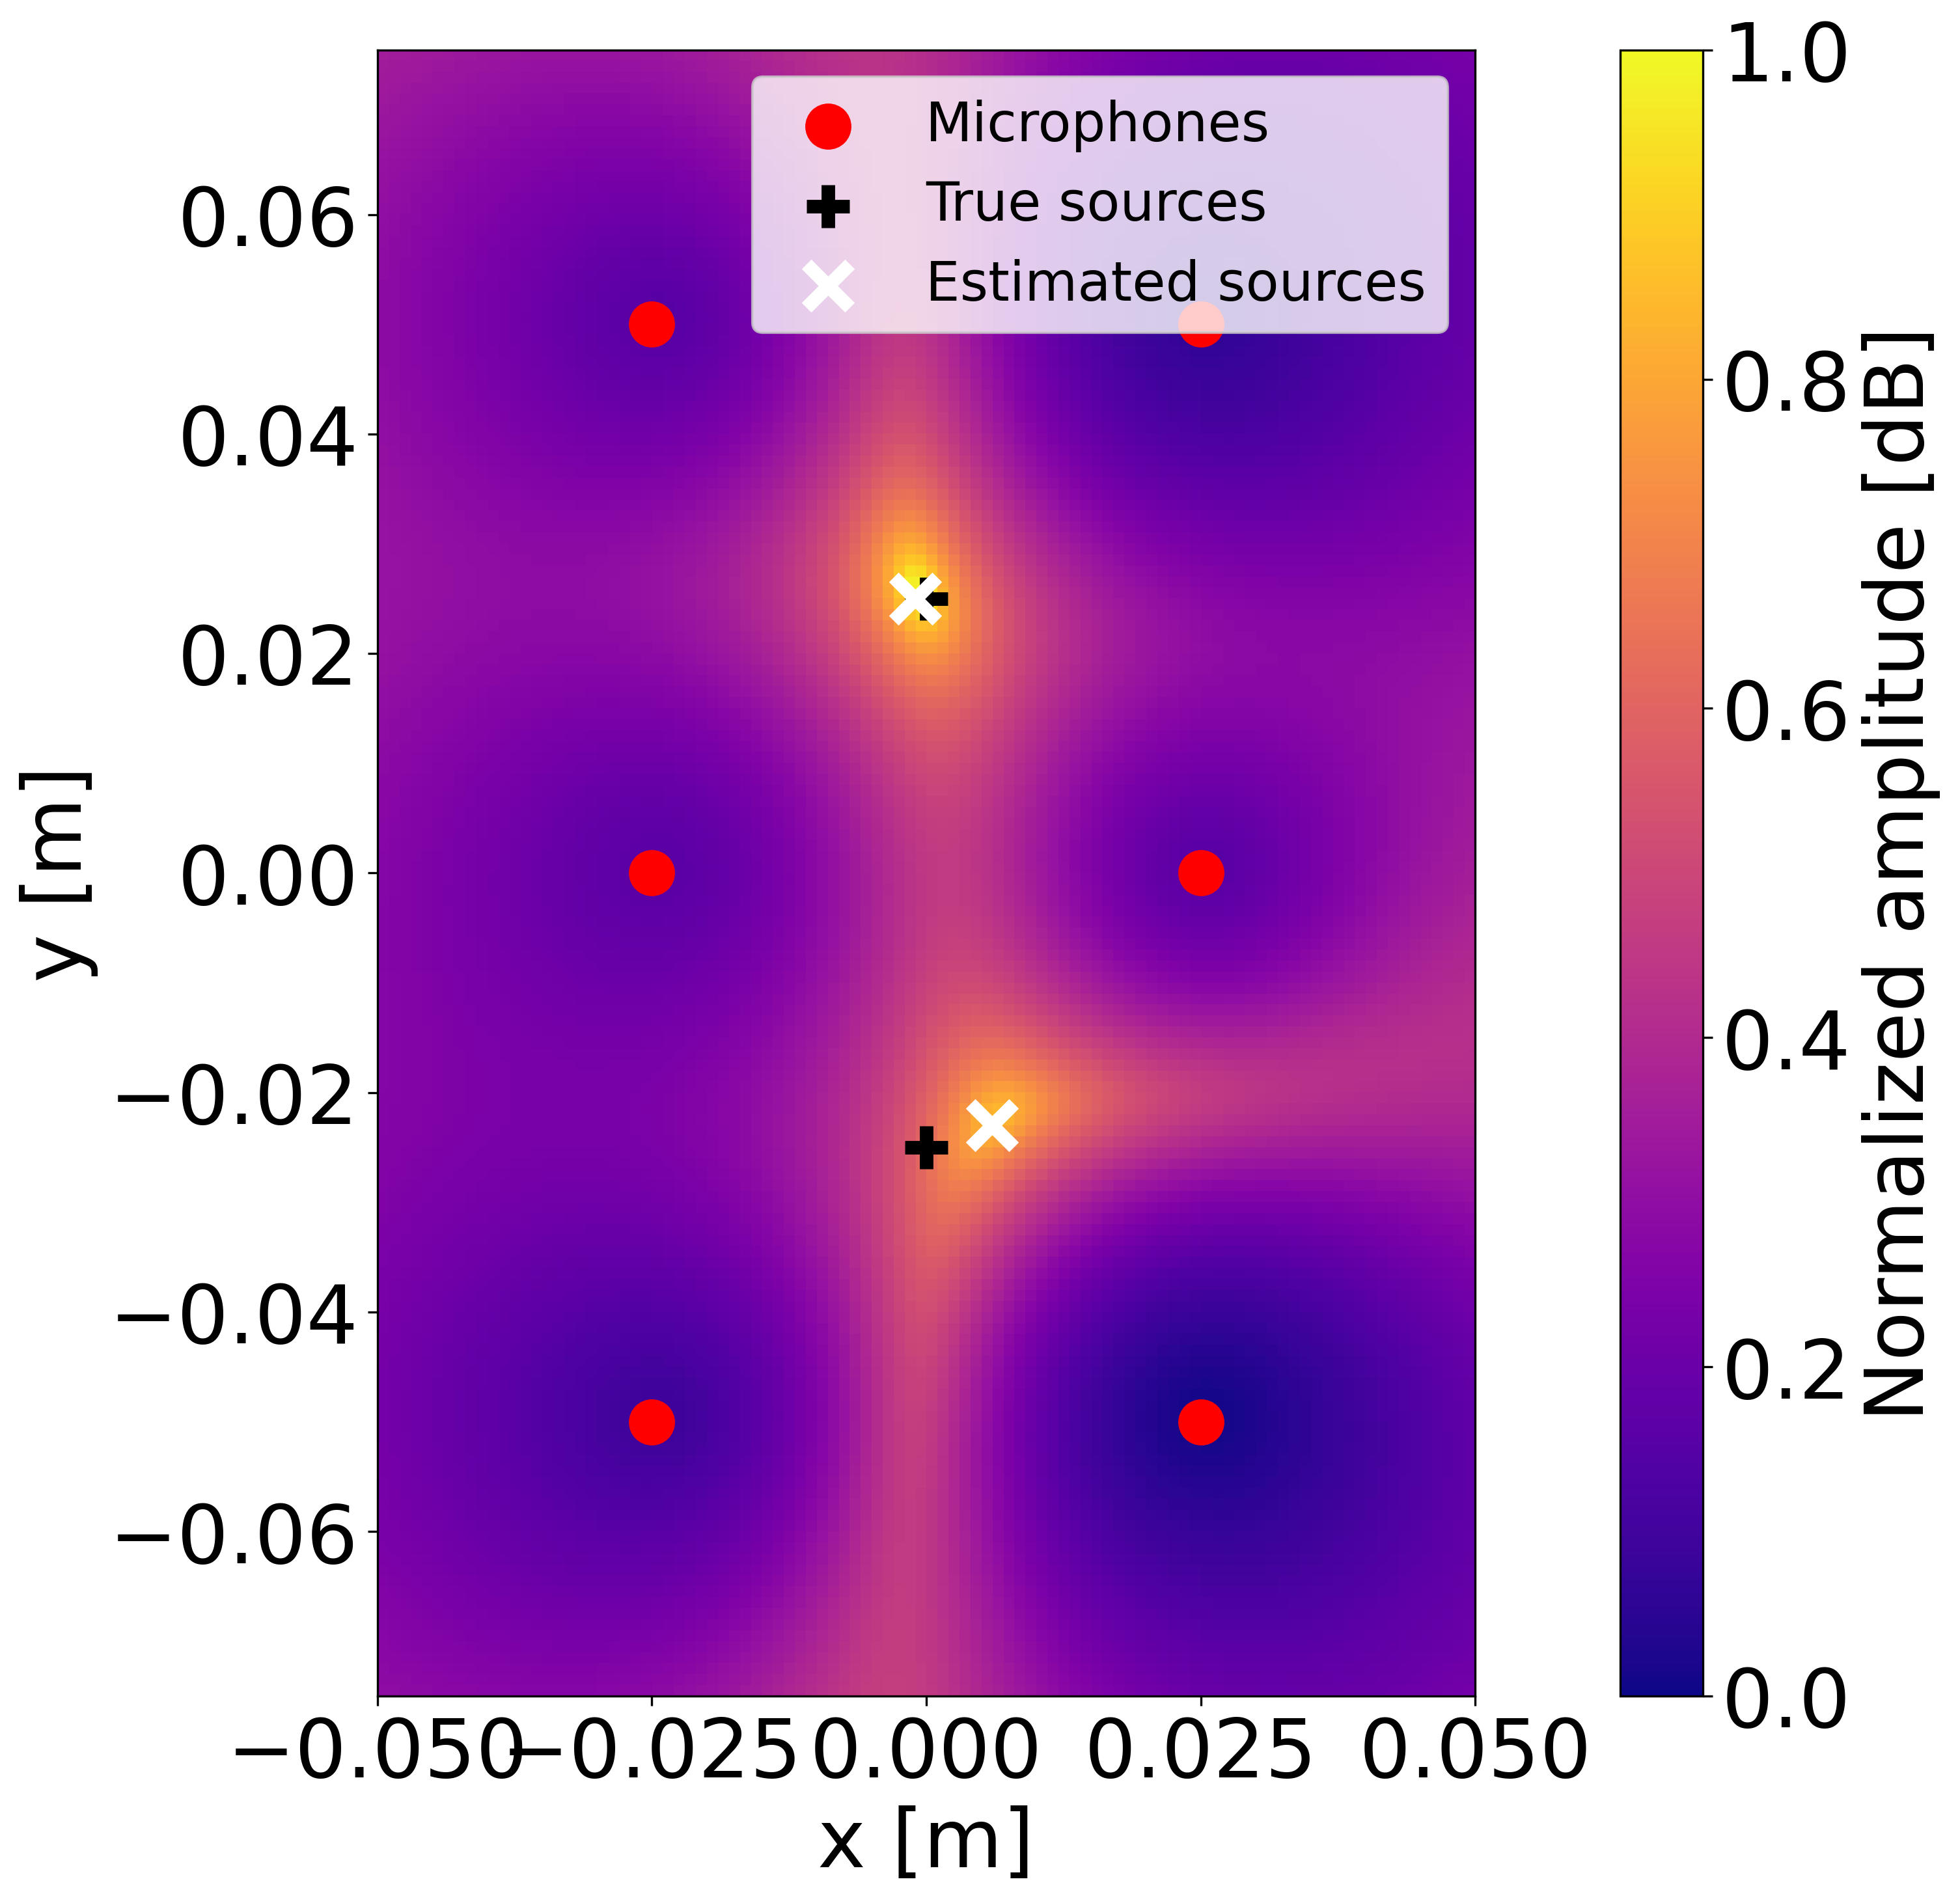
\includegraphics[width=0.6\textwidth]{docs/assignments/Final report/figures/figures/Localization/NEW/Localization_results/Calibrated_MT---_bin0_z1e-05_Fs48000_Q2_M6_v_sound340_d0.1_resolution0.001_modemvdr_neighbourhood3.png}
    \caption{Power plot of the phantom model using 2 sources to simulate the S1 peak using the MVDR algorithm at a depth of 0.00001m.}  
    \label{fig: mvdr_3D_2sources_phantom}
\end{figure}
Although MUSIC is considered as a higher resolution algorithm, it turned out to have similar accuracy to the MVDR. Both have less that a centimeter of error.

\subsection{Human Recordings}
Next, the algorithms were tested by trying to localize the valves or a persons heart. It is not known were the exact locations of the heart valves were, so this is meant as a demonstration. Also the propagation speed of the signal is difficult to be estimated in the tissue, but by varying it there was no significant difference in the results.

\begin{figure} [H]
    \centering
    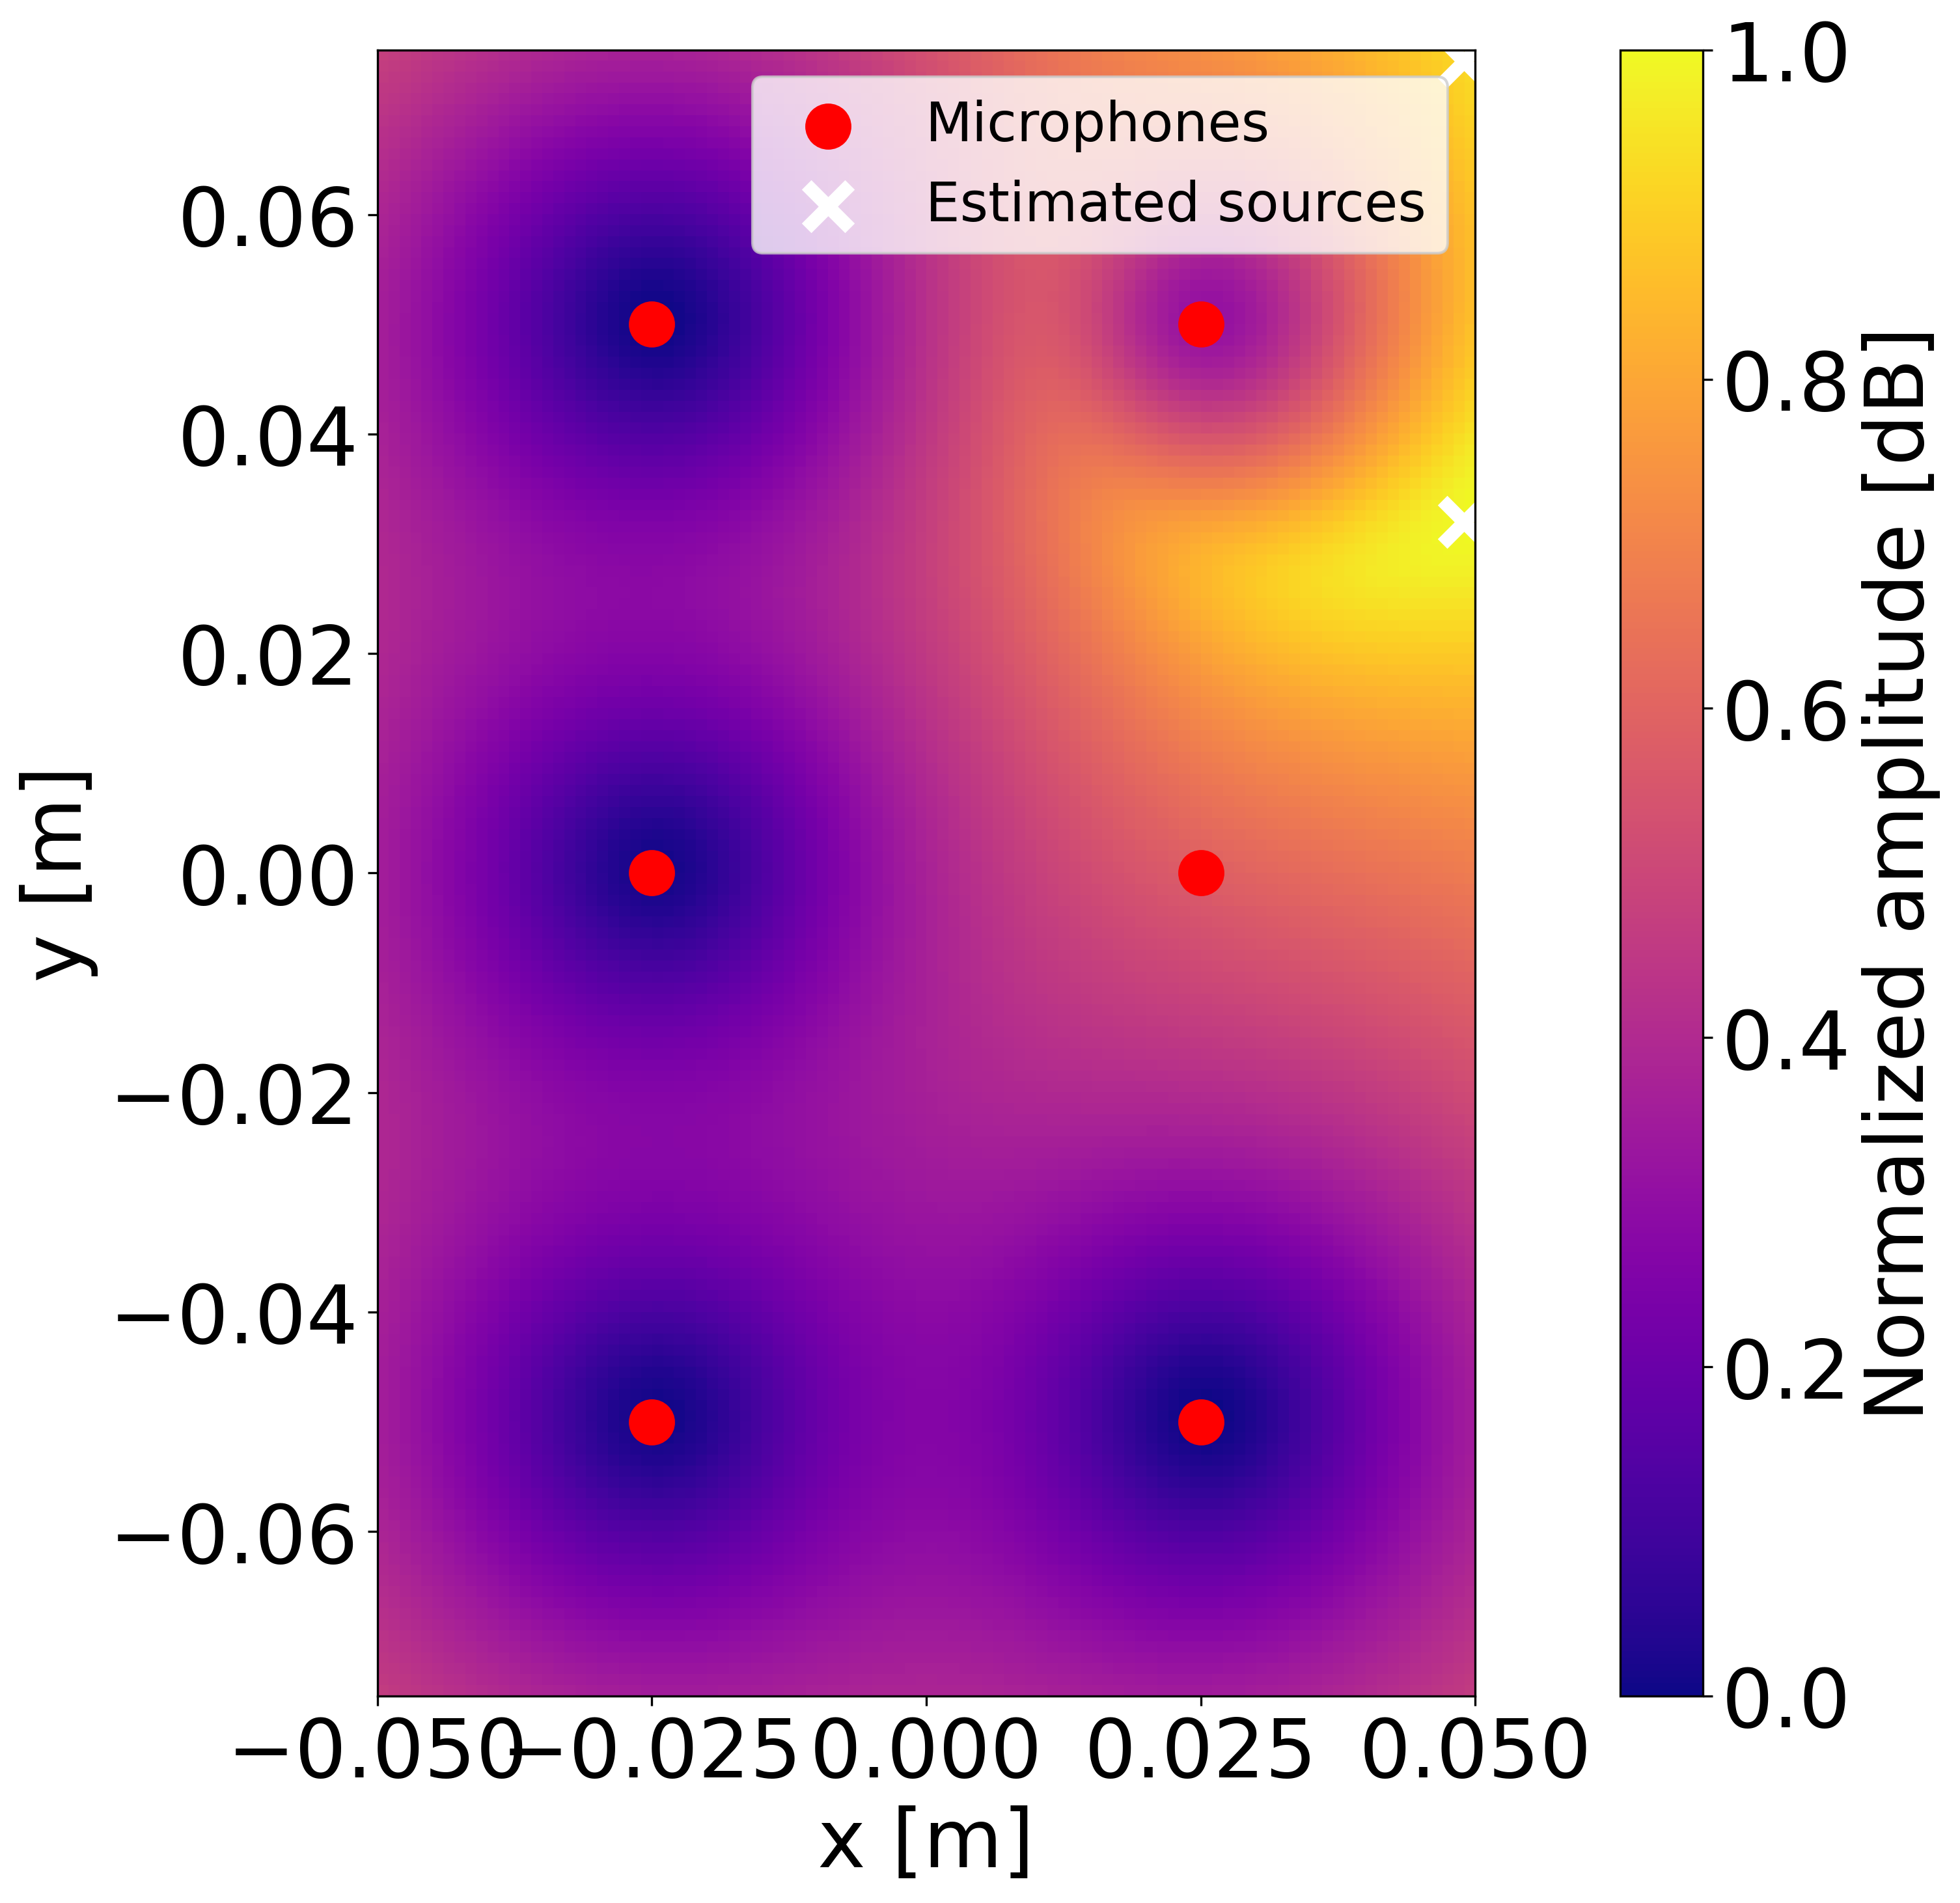
\includegraphics[width=0.6\textwidth]{docs/assignments/Final report/figures/figures/Localization/RealLocalizationResults/real_27cb1086-5d2c-4e5f-b29c-a8c6f9a40b84---_bin0_z0.01_Fs48000_Q2_M6_v_sound340_d0.1_resolution0.001_modemusic_neighbourhood3.png}
    \caption{Power plot of a human recording at a depth of 0.01m using the MUSIC algorithm.}  
    \label{fig: music_3D_2sources_person}
\end{figure}

\begin{figure} [H]
    \centering
    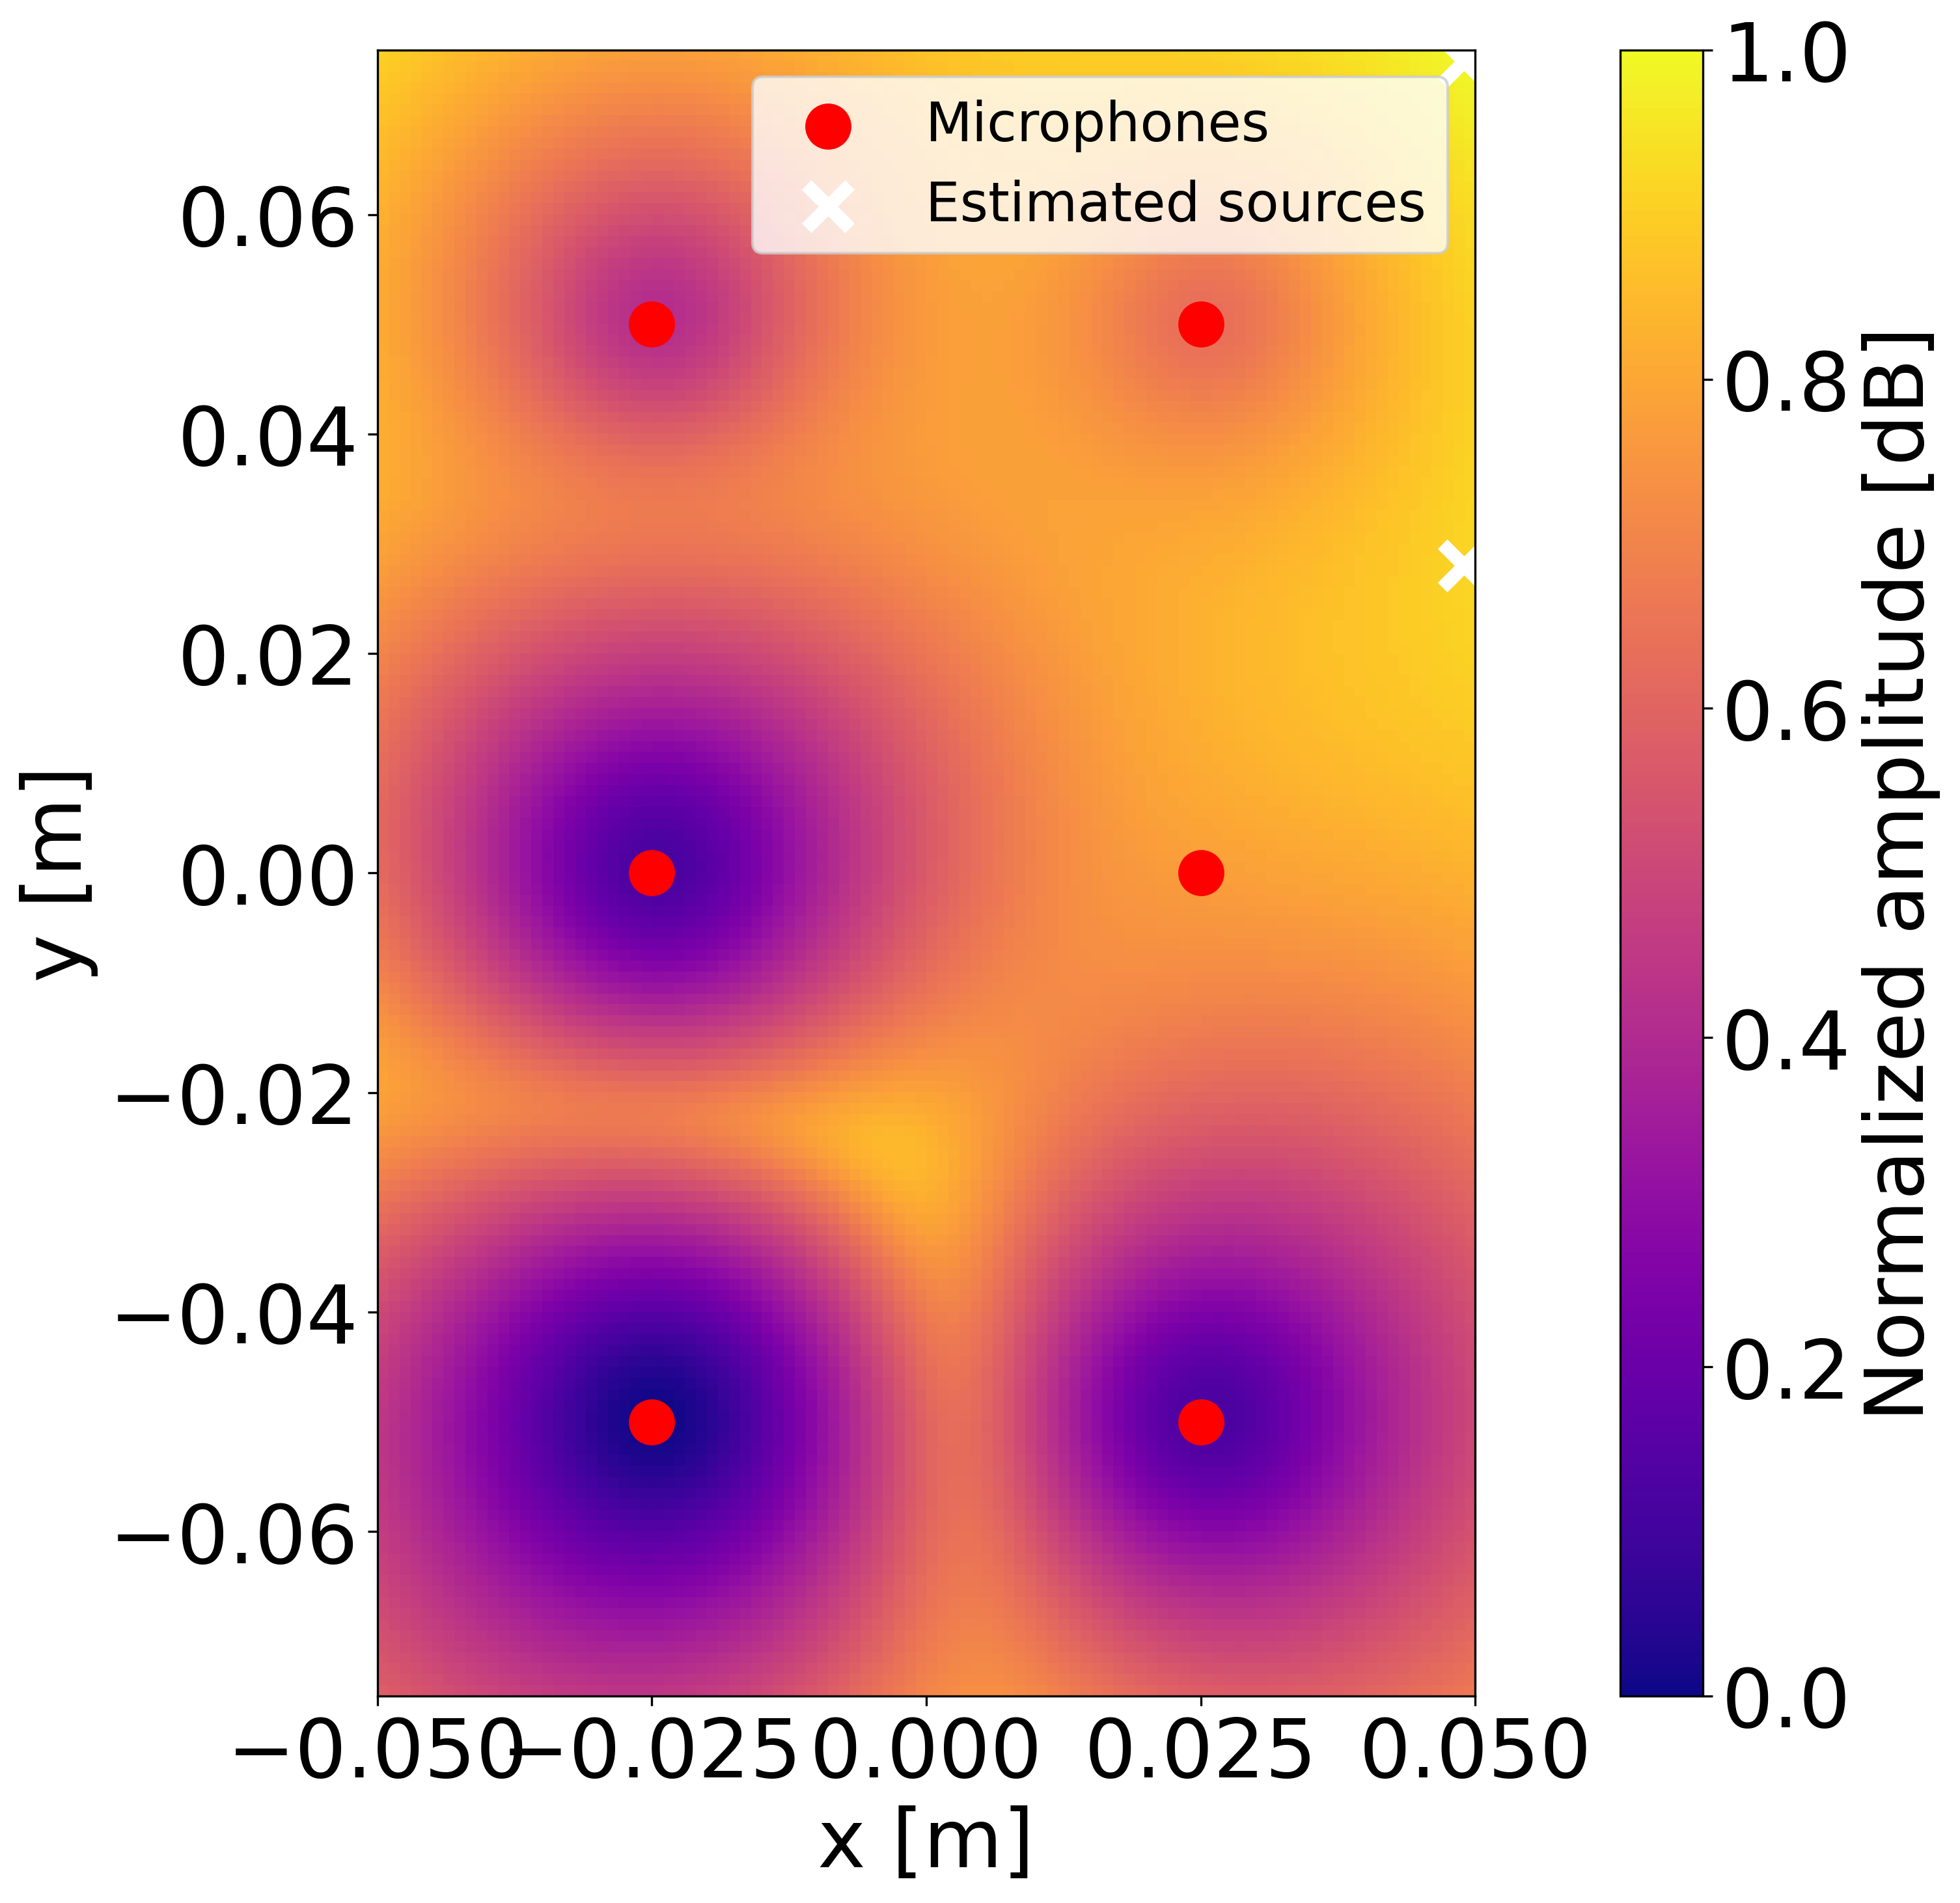
\includegraphics[width=0.6\textwidth]{docs/assignments/Final report/figures/figures/Localization/RealLocalizationResults/real_27cb1086-5d2c-4e5f-b29c-a8c6f9a40b84---_bin0_z0.01_Fs48000_Q2_M6_v_sound340_d0.1_resolution0.001_modemvdr_neighbourhood3.png}
    \caption{Power plot of a human recording at a depth of 0.01m using the MVDR algorithm.}  
    \label{fig: mvdr_3D_2sources_person}
\end{figure}
It can be inferred that both methods give similar results. The only difference is that MUSIC has sharper peaks (thus darker colors further away from the valves) while the MVDR gives a smeared out result, which is expected. It can also been seen that the estimated sources are in the top left of the plot. This is likely due to the microphone array not being placed right above the heart.


\section{Conclusion}
\subsection{Conclusion}
In this chapter, the 2D localization setup was extended to a 3D model that also works in the near field. 
This was done by using a steering vector that depends on the 3D source position instead of only the angle. 
Both MVDR and MUSIC were tested with simulations, phantom recordings, and human recordings.

The simulations show that the method can recover the correct source locations, and that MUSIC gives sharper peaks than MVDR. 
With the phantom model, both methods still worked well even with real noise, and the estimated locations were close to the expected holes in the foam. 
For the human recordings, the exact valve locations are not known, but both methods gave similar and stable localization maps. 
Changing the assumed propagation speed did not strongly change the results.
Overall, the 3D adaptation works and is a useful step toward localizing heart valves.
